\subsection{FRIIS Equation and Shannon-Hartley Capacity}
\subsubsection{FRIIS Equation}
We use FRIIS equation to calculate the \textbf{reception's power}, we use the following parameters:

\begin{align*}
	G_{Tx}= 3dBi\\
	G_{Rx}= 3dBi\\
	c = 3x10^8 \frac{m}{s} \\
	fc = 433MHz\\
	P_{Tx} = 40dBm\\
	Sensibility = -106dBm
\end{align*}

And FRIIS equation:

\begin{equation}
	P_{Rx} = P_{Tx} + G_{Tx} + 20log_{10}(\frac{c}{fc}) -20log(4\pi r)
\end{equation}

We got the next result:

\begin{figure}[!htbp]
	\centering
	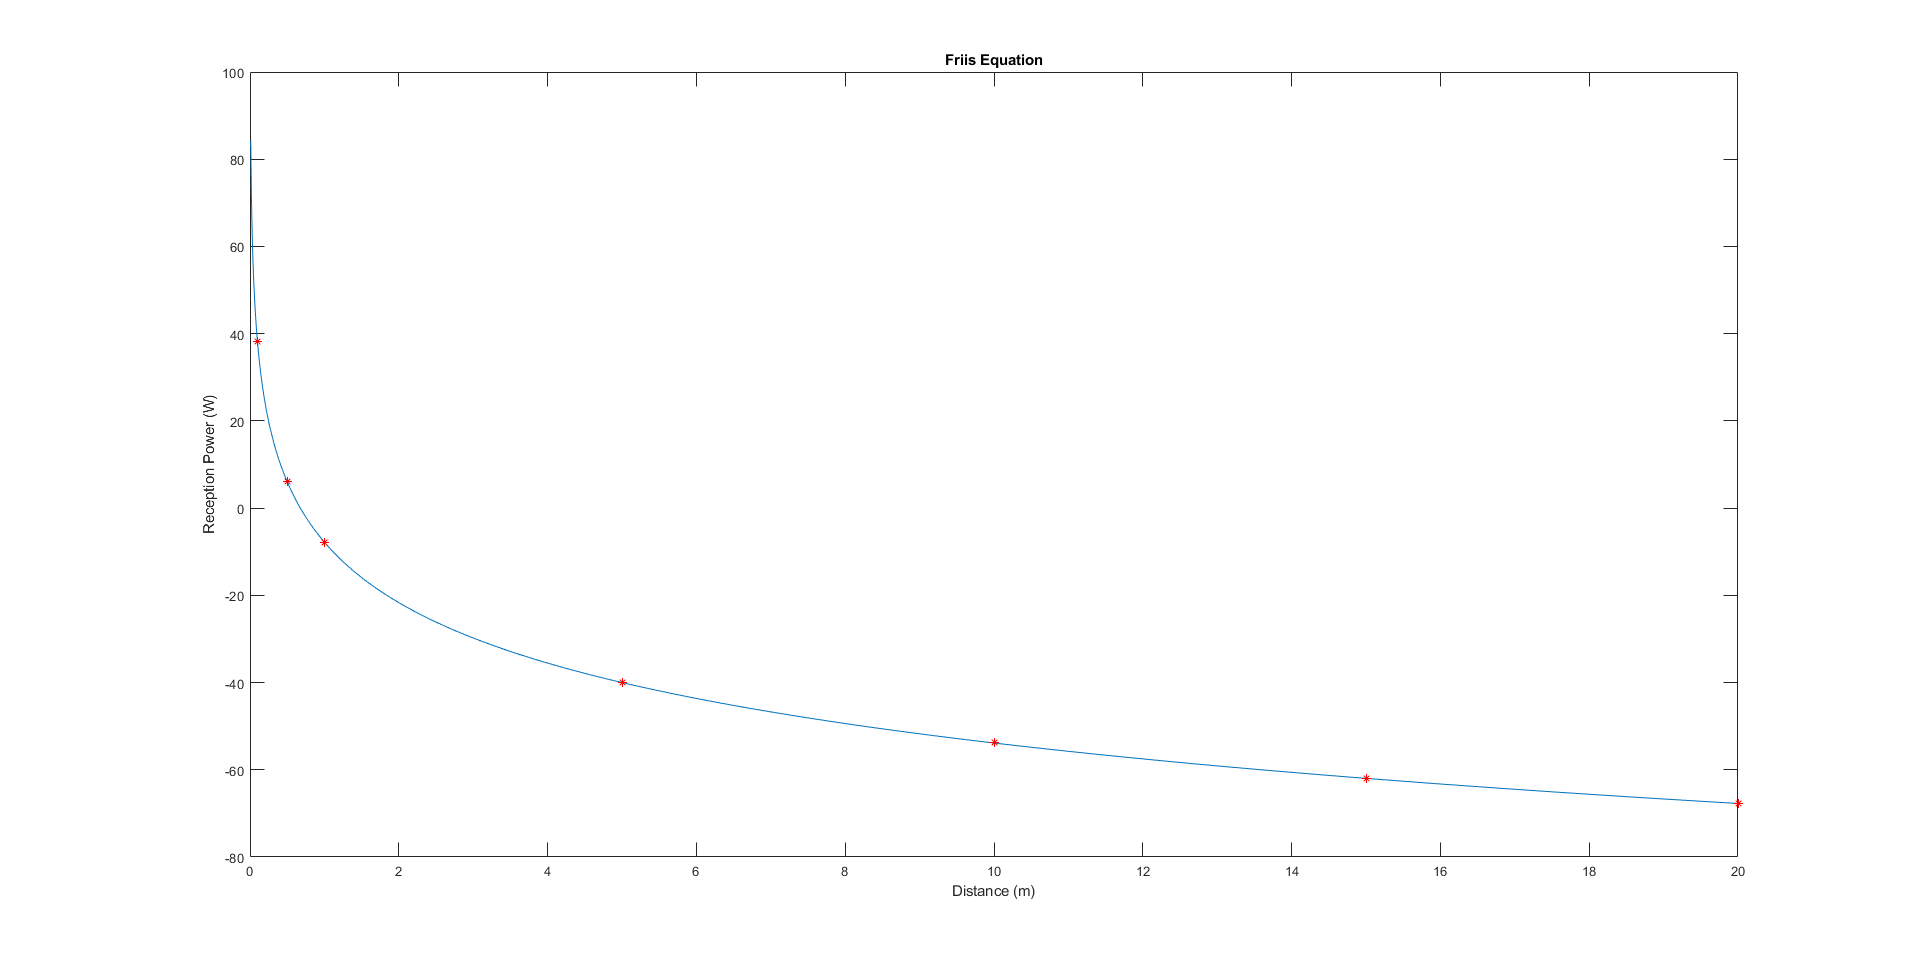
\includegraphics[width=5cm]{images/friis.png}
	\caption{Result of $P_{Tx}$}
\end{figure}

As we can see, our receptor could receive transmission in the distance that we testing because the sensibility is $-106dBm$. But in our testing, show us how the channel disturbed our information while it was travelling.

\subsubsection{Shannon-Hartley Capacity}
We use Shannon-Hartley ecuation to calculate Channel's Capacity. We consider a bandwidth of $25kHz$ because the frecuency operation that we worked using this channel size. %Referencia al doc ese

Shannong-Hartley Capacity Equation
\begin{equation}
	C = Blog_{2}(1+S/N)\\
\end{equation}

We got the next results:

\begin{figure}[!htbp]
	\centering
	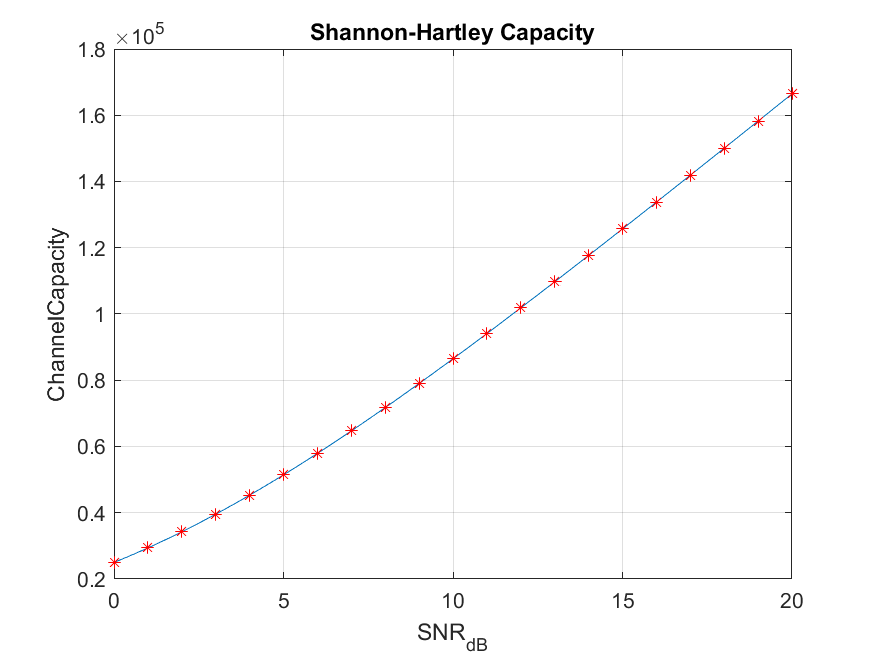
\includegraphics[width=5cm]{images/shannon_capacity.png}
	\caption{Shannon Capacity.}
	\label{fig:shannon}
\end{figure}

Figure \ref{fig:shannon}, show us, as a we expected, while the SNR are increasing, the channel capacity increases, in this practice we noticed that when we separated the transmisor and receptor, because we have another signals interfering like WIFI, LTE, 5G, microwaves, walls, etc. 
